%!TEX root = ./main.tex




\tikzset{every picture/.style={line width=0.75pt}} %set default line width to 0.75pt        

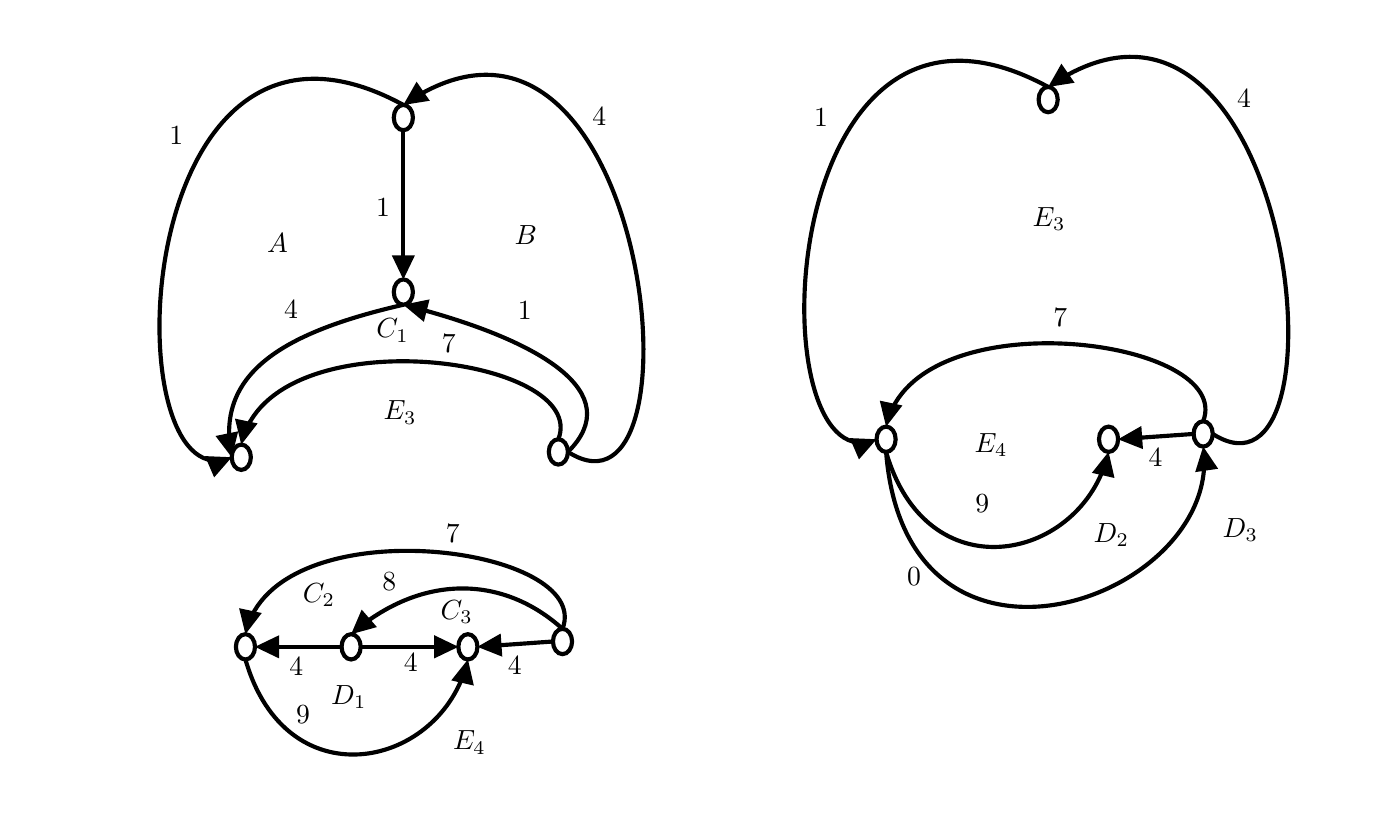
\begin{tikzpicture}[x=0.75pt,y=0.75pt,yscale=-1,xscale=1]
%uncomment if require: \path (0,498); %set diagram left start at 0, and has height of 498
\path[use as bounding box] (20,10) rectangle (660,380);
%Shape: Ellipse [id:dp35589263376995484] 
\draw  [color={rgb, 255:red, 0; green, 0; blue, 0 }  ,draw opacity=1 ][line width=1.5]  (507.06,44.65) .. controls (507.06,41.28) and (509.12,38.55) .. (511.67,38.55) .. controls (514.21,38.55) and (516.27,41.28) .. (516.27,44.65) .. controls (516.27,48.02) and (514.21,50.75) .. (511.67,50.75) .. controls (509.12,50.75) and (507.06,48.02) .. (507.06,44.65) -- cycle ;
%Shape: Ellipse [id:dp5273685537709042] 
\draw  [color={rgb, 255:red, 0; green, 0; blue, 0 }  ,draw opacity=1 ][line width=1.5]  (428.98,208.3) .. controls (428.98,204.94) and (431.04,202.21) .. (433.59,202.21) .. controls (436.13,202.21) and (438.19,204.94) .. (438.19,208.3) .. controls (438.19,211.67) and (436.13,214.4) .. (433.59,214.4) .. controls (431.04,214.4) and (428.98,211.67) .. (428.98,208.3) -- cycle ;
%Shape: Ellipse [id:dp9933087224039621] 
\draw  [color={rgb, 255:red, 0; green, 0; blue, 0 }  ,draw opacity=1 ][line width=1.5]  (581.74,205.74) .. controls (581.74,202.37) and (583.8,199.64) .. (586.35,199.64) .. controls (588.89,199.64) and (590.96,202.37) .. (590.96,205.74) .. controls (590.96,209.1) and (588.89,211.83) .. (586.35,211.83) .. controls (583.8,211.83) and (581.74,209.1) .. (581.74,205.74) -- cycle ;
%Shape: Ellipse [id:dp4223187867652599] 
\draw  [color={rgb, 255:red, 0; green, 0; blue, 0 }  ,draw opacity=1 ][line width=1.5]  (536.16,208.3) .. controls (536.16,204.94) and (538.22,202.21) .. (540.76,202.21) .. controls (543.31,202.21) and (545.37,204.94) .. (545.37,208.3) .. controls (545.37,211.67) and (543.31,214.4) .. (540.76,214.4) .. controls (538.22,214.4) and (536.16,211.67) .. (536.16,208.3) -- cycle ;
%Curve Lines [id:da32707407117974907] 
\draw [color={rgb, 255:red, 0; green, 0; blue, 0 }  ,draw opacity=1 ][line width=1.5]    (590.96,205.74) .. controls (659.24,249.16) and (630.29,-40.35) .. (513.43,37.36) ;
\draw [shift={(511.67,38.55)}, rotate = 325.34] [fill={rgb, 255:red, 0; green, 0; blue, 0 }  ,fill opacity=1 ][line width=0.08]  [draw opacity=0] (11.61,-5.58) -- (0,0) -- (11.61,5.58) -- cycle    ;
%Curve Lines [id:da7020868150054066] 
\draw [color={rgb, 255:red, 0; green, 0; blue, 0 }  ,draw opacity=1 ][line width=1.5]    (424.72,209.64) .. controls (370.98,220.16) and (381.16,-32.47) .. (511.67,38.55) ;
\draw [shift={(428.98,208.3)}, rotate = 156.81] [fill={rgb, 255:red, 0; green, 0; blue, 0 }  ,fill opacity=1 ][line width=0.08]  [draw opacity=0] (11.61,-5.58) -- (0,0) -- (11.61,5.58) -- cycle    ;
%Straight Lines [id:da6734901748040498] 
\draw [color={rgb, 255:red, 0; green, 0; blue, 0 }  ,draw opacity=1 ][line width=1.5]    (549.36,208.02) -- (581.74,205.74) ;
\draw [shift={(545.37,208.3)}, rotate = 355.96] [fill={rgb, 255:red, 0; green, 0; blue, 0 }  ,fill opacity=1 ][line width=0.08]  [draw opacity=0] (11.61,-5.58) -- (0,0) -- (11.61,5.58) -- cycle    ;
%Curve Lines [id:da03703637046060837] 
\draw [line width=1.5]    (586.35,199.64) .. controls (601.62,160.02) and (453,140.46) .. (434.55,198.55) ;
\draw [shift={(433.59,202.21)}, rotate = 281.99] [fill={rgb, 255:red, 0; green, 0; blue, 0 }  ][line width=0.08]  [draw opacity=0] (11.61,-5.58) -- (0,0) -- (11.61,5.58) -- cycle    ;
%Curve Lines [id:da798612936169141] 
\draw [line width=1.5]    (433.59,214.4) .. controls (453.03,281.98) and (525.13,267.42) .. (539.75,218.25) ;
\draw [shift={(540.76,214.4)}, rotate = 102.83] [fill={rgb, 255:red, 0; green, 0; blue, 0 }  ][line width=0.08]  [draw opacity=0] (11.61,-5.58) -- (0,0) -- (11.61,5.58) -- cycle    ;
%Curve Lines [id:da8888761441506123] 
\draw [line width=1.5]    (433.59,214.4) .. controls (443.17,338.24) and (592.39,286.2) .. (586.72,215.09) ;
\draw [shift={(586.35,211.83)}, rotate = 81.69] [fill={rgb, 255:red, 0; green, 0; blue, 0 }  ][line width=0.08]  [draw opacity=0] (11.61,-5.58) -- (0,0) -- (11.61,5.58) -- cycle    ;
%Shape: Ellipse [id:dp8150638560518382] 
\draw  [color={rgb, 255:red, 0; green, 0; blue, 0 }  ,draw opacity=1 ][line width=1.5]  (196.39,53.32) .. controls (196.39,49.95) and (198.45,47.22) .. (201,47.22) .. controls (203.54,47.22) and (205.61,49.95) .. (205.61,53.32) .. controls (205.61,56.69) and (203.54,59.41) .. (201,59.41) .. controls (198.45,59.41) and (196.39,56.69) .. (196.39,53.32) -- cycle ;
%Shape: Ellipse [id:dp07405350698131474] 
\draw  [color={rgb, 255:red, 0; green, 0; blue, 0 }  ,draw opacity=1 ][line width=1.5]  (196.39,137.39) .. controls (196.39,134.02) and (198.45,131.29) .. (201,131.29) .. controls (203.54,131.29) and (205.61,134.02) .. (205.61,137.39) .. controls (205.61,140.76) and (203.54,143.49) .. (201,143.49) .. controls (198.45,143.49) and (196.39,140.76) .. (196.39,137.39) -- cycle ;
%Curve Lines [id:da5729143394323514] 
\draw [color={rgb, 255:red, 0; green, 0; blue, 0 }  ,draw opacity=1 ][line width=1.5]    (117.61,212.9) .. controls (112.41,176.16) and (142.97,156.8) .. (201,143.49) ;
\draw [shift={(118.31,216.97)}, rotate = 258.41] [fill={rgb, 255:red, 0; green, 0; blue, 0 }  ,fill opacity=1 ][line width=0.08]  [draw opacity=0] (11.61,-5.58) -- (0,0) -- (11.61,5.58) -- cycle    ;
%Curve Lines [id:da985022859832252] 
\draw [color={rgb, 255:red, 0; green, 0; blue, 0 }  ,draw opacity=1 ][line width=1.5]    (280.29,214.4) .. controls (308.81,186.1) and (267.69,160.88) .. (204.87,144.48) ;
\draw [shift={(201,143.49)}, rotate = 14.13] [fill={rgb, 255:red, 0; green, 0; blue, 0 }  ,fill opacity=1 ][line width=0.08]  [draw opacity=0] (11.61,-5.58) -- (0,0) -- (11.61,5.58) -- cycle    ;
%Curve Lines [id:da42144751436003447] 
\draw [color={rgb, 255:red, 0; green, 0; blue, 0 }  ,draw opacity=1 ][line width=1.5]    (280.29,214.4) .. controls (348.57,257.82) and (319.62,-31.69) .. (202.77,46.02) ;
\draw [shift={(201,47.22)}, rotate = 325.34] [fill={rgb, 255:red, 0; green, 0; blue, 0 }  ,fill opacity=1 ][line width=0.08]  [draw opacity=0] (11.61,-5.58) -- (0,0) -- (11.61,5.58) -- cycle    ;
%Curve Lines [id:da7830144424190421] 
\draw [color={rgb, 255:red, 0; green, 0; blue, 0 }  ,draw opacity=1 ][line width=1.5]    (114.05,218.31) .. controls (60.32,228.83) and (70.5,-23.8) .. (201,47.22) ;
\draw [shift={(118.31,216.97)}, rotate = 156.81] [fill={rgb, 255:red, 0; green, 0; blue, 0 }  ,fill opacity=1 ][line width=0.08]  [draw opacity=0] (11.61,-5.58) -- (0,0) -- (11.61,5.58) -- cycle    ;
%Straight Lines [id:da11394903068946982] 
\draw [color={rgb, 255:red, 0; green, 0; blue, 0 }  ,draw opacity=1 ][line width=1.5]    (201,127.29) -- (201,59.41) ;
\draw [shift={(201,131.29)}, rotate = 270] [fill={rgb, 255:red, 0; green, 0; blue, 0 }  ,fill opacity=1 ][line width=0.08]  [draw opacity=0] (11.61,-5.58) -- (0,0) -- (11.61,5.58) -- cycle    ;
%Curve Lines [id:da9079411866287189] 
\draw [line width=1.5]    (275.68,208.31) .. controls (290.96,168.68) and (142.33,149.13) .. (123.88,207.22) ;
\draw [shift={(122.92,210.87)}, rotate = 281.99] [fill={rgb, 255:red, 0; green, 0; blue, 0 }  ][line width=0.08]  [draw opacity=0] (11.61,-5.58) -- (0,0) -- (11.61,5.58) -- cycle    ;
%Shape: Ellipse [id:dp9797878316847205] 
\draw  [color={rgb, 255:red, 0; green, 0; blue, 0 }  ,draw opacity=1 ][line width=1.5]  (271.08,214.4) .. controls (271.08,211.03) and (273.14,208.31) .. (275.68,208.31) .. controls (278.23,208.31) and (280.29,211.03) .. (280.29,214.4) .. controls (280.29,217.77) and (278.23,220.5) .. (275.68,220.5) .. controls (273.14,220.5) and (271.08,217.77) .. (271.08,214.4) -- cycle ;
%Shape: Ellipse [id:dp11924297827138353] 
\draw  [color={rgb, 255:red, 0; green, 0; blue, 0 }  ,draw opacity=1 ][line width=1.5]  (120.31,308.3) .. controls (120.31,304.94) and (122.38,302.21) .. (124.92,302.21) .. controls (127.46,302.21) and (129.53,304.94) .. (129.53,308.3) .. controls (129.53,311.67) and (127.46,314.4) .. (124.92,314.4) .. controls (122.38,314.4) and (120.31,311.67) .. (120.31,308.3) -- cycle ;
%Shape: Ellipse [id:dp18019428491254885] 
\draw  [color={rgb, 255:red, 0; green, 0; blue, 0 }  ,draw opacity=1 ][line width=1.5]  (118.31,216.97) .. controls (118.31,213.6) and (120.38,210.87) .. (122.92,210.87) .. controls (125.46,210.87) and (127.53,213.6) .. (127.53,216.97) .. controls (127.53,220.34) and (125.46,223.07) .. (122.92,223.07) .. controls (120.38,223.07) and (118.31,220.34) .. (118.31,216.97) -- cycle ;
%Shape: Ellipse [id:dp2447839509836378] 
\draw  [color={rgb, 255:red, 0; green, 0; blue, 0 }  ,draw opacity=1 ][line width=1.5]  (171.23,308.3) .. controls (171.23,304.94) and (173.3,302.21) .. (175.84,302.21) .. controls (178.39,302.21) and (180.45,304.94) .. (180.45,308.3) .. controls (180.45,311.67) and (178.39,314.4) .. (175.84,314.4) .. controls (173.3,314.4) and (171.23,311.67) .. (171.23,308.3) -- cycle ;
%Shape: Ellipse [id:dp33013962263442154] 
\draw  [color={rgb, 255:red, 0; green, 0; blue, 0 }  ,draw opacity=1 ][line width=1.5]  (227.49,308.3) .. controls (227.49,304.94) and (229.55,302.21) .. (232.1,302.21) .. controls (234.64,302.21) and (236.7,304.94) .. (236.7,308.3) .. controls (236.7,311.67) and (234.64,314.4) .. (232.1,314.4) .. controls (229.55,314.4) and (227.49,311.67) .. (227.49,308.3) -- cycle ;
%Straight Lines [id:da31396117550667135] 
\draw [color={rgb, 255:red, 0; green, 0; blue, 0 }  ,draw opacity=1 ][line width=1.5]    (133.53,308.3) -- (171.23,308.3) ;
\draw [shift={(129.53,308.3)}, rotate = 0] [fill={rgb, 255:red, 0; green, 0; blue, 0 }  ,fill opacity=1 ][line width=0.08]  [draw opacity=0] (11.61,-5.58) -- (0,0) -- (11.61,5.58) -- cycle    ;
%Straight Lines [id:da6005265572468635] 
\draw [color={rgb, 255:red, 0; green, 0; blue, 0 }  ,draw opacity=1 ][line width=1.5]    (180.45,308.3) -- (223.49,308.3) ;
\draw [shift={(227.49,308.3)}, rotate = 180] [fill={rgb, 255:red, 0; green, 0; blue, 0 }  ,fill opacity=1 ][line width=0.08]  [draw opacity=0] (11.61,-5.58) -- (0,0) -- (11.61,5.58) -- cycle    ;
%Straight Lines [id:da1808031690077344] 
\draw [color={rgb, 255:red, 0; green, 0; blue, 0 }  ,draw opacity=1 ][line width=1.5]    (240.69,308.02) -- (273.08,305.74) ;
\draw [shift={(236.7,308.3)}, rotate = 355.96] [fill={rgb, 255:red, 0; green, 0; blue, 0 }  ,fill opacity=1 ][line width=0.08]  [draw opacity=0] (11.61,-5.58) -- (0,0) -- (11.61,5.58) -- cycle    ;
%Curve Lines [id:da3357677157773651] 
\draw [line width=1.5]    (277.68,299.64) .. controls (292.96,260.02) and (144.33,240.46) .. (125.88,298.55) ;
\draw [shift={(124.92,302.21)}, rotate = 281.99] [fill={rgb, 255:red, 0; green, 0; blue, 0 }  ][line width=0.08]  [draw opacity=0] (11.61,-5.58) -- (0,0) -- (11.61,5.58) -- cycle    ;
%Curve Lines [id:da670250481056926] 
\draw [line width=1.5]    (179.35,299.27) .. controls (211.8,273.31) and (249.51,274.2) .. (277.68,299.64) ;
\draw [shift={(175.84,302.21)}, rotate = 318.94] [fill={rgb, 255:red, 0; green, 0; blue, 0 }  ][line width=0.08]  [draw opacity=0] (11.61,-5.58) -- (0,0) -- (11.61,5.58) -- cycle    ;
%Curve Lines [id:da1585249402391844] 
\draw [line width=1.5]    (124.92,314.4) .. controls (144.36,381.98) and (216.47,367.42) .. (231.09,318.25) ;
\draw [shift={(232.1,314.4)}, rotate = 102.83] [fill={rgb, 255:red, 0; green, 0; blue, 0 }  ][line width=0.08]  [draw opacity=0] (11.61,-5.58) -- (0,0) -- (11.61,5.58) -- cycle    ;
%Shape: Ellipse [id:dp8849254018327529] 
\draw  [color={rgb, 255:red, 0; green, 0; blue, 0 }  ,draw opacity=1 ][line width=1.5]  (273.08,305.74) .. controls (273.08,302.37) and (275.14,299.64) .. (277.68,299.64) .. controls (280.23,299.64) and (282.29,302.37) .. (282.29,305.74) .. controls (282.29,309.1) and (280.23,311.83) .. (277.68,311.83) .. controls (275.14,311.83) and (273.08,309.1) .. (273.08,305.74) -- cycle ;

% Text Node
\draw (601.26,38.41) node [anchor=north west][inner sep=0.75pt]    {$4$};
% Text Node
\draw (397.44,47.33) node [anchor=north west][inner sep=0.75pt]    {$1$};
% Text Node
\draw (558.52,211.43) node [anchor=north west][inner sep=0.75pt]    {$4$};
% Text Node
\draw (532.09,247.38) node [anchor=north west][inner sep=0.75pt]    {$D_{2}$};
% Text Node
\draw (594.24,244.82) node [anchor=north west][inner sep=0.75pt]    {$D_{3}$};
% Text Node
\draw (442.27,268.73) node [anchor=north west][inner sep=0.75pt]    {$0$};
% Text Node
\draw (133.88,107.84) node [anchor=north west][inner sep=0.75pt]    {$A$};
% Text Node
\draw (253.06,103.72) node [anchor=north west][inner sep=0.75pt]    {$B$};
% Text Node
\draw (290.6,47.07) node [anchor=north west][inner sep=0.75pt]    {$4$};
% Text Node
\draw (142.03,140.11) node [anchor=north west][inner sep=0.75pt]    {$4$};
% Text Node
\draw (254.63,140.45) node [anchor=north west][inner sep=0.75pt]    {$1$};
% Text Node
\draw (86.77,56) node [anchor=north west][inner sep=0.75pt]    {$1$};
% Text Node
\draw (186.34,90.67) node [anchor=north west][inner sep=0.75pt]    {$1$};
% Text Node
\draw (186.56,148.89) node [anchor=north west][inner sep=0.75pt]    {$C_{1}$};
% Text Node
\draw (218.02,156.44) node [anchor=north west][inner sep=0.75pt]    {$7$};
% Text Node
\draw (190,188.4) node [anchor=north west][inner sep=0.75pt]    {$E_{3}$};
% Text Node
\draw (144.55,312.12) node [anchor=north west][inner sep=0.75pt]    {$4$};
% Text Node
\draw (199.81,310.06) node [anchor=north west][inner sep=0.75pt]    {$4$};
% Text Node
\draw (249.85,311.43) node [anchor=north west][inner sep=0.75pt]    {$4$};
% Text Node
\draw (217.5,284.38) node [anchor=north west][inner sep=0.75pt]    {$C_{3}$};
% Text Node
\draw (151.1,276.12) node [anchor=north west][inner sep=0.75pt]    {$C_{2}$};
% Text Node
\draw (220.02,247.77) node [anchor=north west][inner sep=0.75pt]    {$7$};
% Text Node
\draw (189.37,271.13) node [anchor=north west][inner sep=0.75pt]    {$8$};
% Text Node
\draw (164.69,325.59) node [anchor=north west][inner sep=0.75pt]    {$D_{1}$};
% Text Node
\draw (223.43,347.38) node [anchor=north west][inner sep=0.75pt]    {$E_{4}$};
% Text Node
\draw (147.8,335.38) node [anchor=north west][inner sep=0.75pt]    {$9$};
% Text Node
\draw (512.68,143.77) node [anchor=north west][inner sep=0.75pt]    {$7$};
% Text Node
\draw (502.67,95.07) node [anchor=north west][inner sep=0.75pt]    {$E_{3}$};
% Text Node
\draw (475.13,233.38) node [anchor=north west][inner sep=0.75pt]    {$9$};
% Text Node
\draw (474.76,204.05) node [anchor=north west][inner sep=0.75pt]    {$E_{4}$};


\end{tikzpicture}